\documentclass[xcolor=svgnames]{beamer}
\usetheme{Boadilla}
\usecolortheme[named=ForestGreen]{structure}
\usepackage{graphicx}
\usepackage[final]{animate}
%\usepackage[colorlinks=true,urlcolor=blue,citecolor=blue,linkcolor=blue]{hyperref}
\usepackage{breqn}
\usepackage{xcolor}
\usepackage{booktabs}
\usepackage{tikz}
\usetikzlibrary{shadows,arrows,positioning}
\usepackage[noae]{Sweave}
\definecolor{links}{HTML}{2A1B81}
\hypersetup{colorlinks,linkcolor=links,urlcolor=links}
\usepackage{pgfpages}
%\pgfpagesuselayout{4 on 1}[letterpaper, border shrink = 5mm, landscape]

\tikzstyle{block} = [rectangle, draw, text width=7em, text centered, rounded corners, minimum height=3em, minimum width=7em, top color = white, bottom color=green!30,  drop shadow]

\begin{document}
\SweaveOpts{concordance=TRUE}

\title[R for Data Analysis]{\includegraphics[width=0.07\textwidth]{Rlogo.jpg} \hspace{0.2em} for Data Analysis}
\author[M. Beck and S. Berg]{Marcus W. Beck \and Sergey Berg}

\institute[UofM]{Department of Fisheries, Wildlife, and Conservation Biology \\ University of Minnesota, Twin Cities}

\date{May 21, 2013}

\titlegraphic{
\centerline{
\begin{tikzpicture}
  \node[fill=white,draw] at (0,0) {\includegraphics[width=0.6\textwidth]{peeper.jpg}};
\end{tikzpicture}}
}

%%%%%%
\begin{frame}
\vspace{-0.3in}
\titlepage
\end{frame}

\section{Background}

%%%%%%
\begin{frame}{What you'll learn about \hspace{0.2em}\includegraphics[width=0.07\textwidth]{Rlogo.jpg}}
\setbeamercovered{again covered={\opaqueness<1->{25}}}
\onslide<1->
\begin{itemize}
\itemsep20pt
\item Data organization
\item Data exploration and visualization
\begin{itemize}
\item Common functions
\item Graphing tools
\end{itemize}
\item Data analysis and hypothesis testing
\begin{itemize}
\item Common functions
\item Evaluation of output 
\item Graphing tools \\~\\
\end{itemize}
\end{itemize}
\pause
\Large
\centerline{\emph{Interactive! Interrupt me!}}
\end{frame}

\section{Data organization}

%%%%%%
\begin{frame}[fragile]{Data organization}
We'll use the same dataset we used in Excel, replicating the analyses\\~\\
First we have to import the data into our R `workspace' \\~\\
\pause
The workspace is a group of R objects that are loaded for our current session \\~\\
Data are loaded into the workspace by importing (or making within R) and assigning them to a variable (object) with a name of our choosing\\~\\
We can see what's loaded in our workspace:\\~\\
\pause
<<echo=true>>=
a<-c(1,2)
ls()
@
\end{frame}

%%%%%%
\begin{frame}[fragile]{Data organization}
\onslide<+->{Import the data following this workflow:}\\~\\
\begin{center}
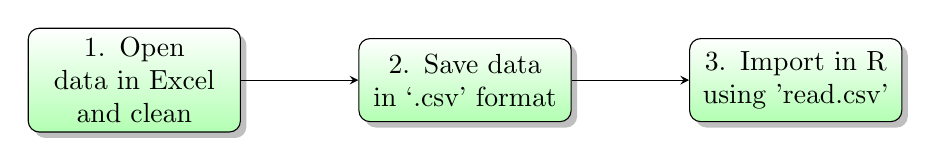
\begin{tikzpicture}[node distance=2.5cm, auto, >=stealth]
	\onslide<2->{
	\node[block] (a) {1. Open data in Excel and clean};}
	\onslide<3->{
	\node[block] (b)  [right of=a, node distance=4.2cm] {2. Save data in `.csv' format};
 	\draw[->] (a) -- (b);}
 	\onslide<4->{
 	\node[block] (c)  [right of=b, node distance=4.2cm]  {3. Import in R using 'read.csv'};
 	\draw[->] (b) -- (c);}
\end{tikzpicture}
\end{center}
\begin{columns}[t]
\onslide<2->{
\begin{column}{0.33\textwidth}
\begin{itemize}
\item Column names should be simple
\item Ensure all data will be easy to read
\end{itemize}
\end{column}}
\onslide<3->{
\begin{column}{0.33\textwidth}
\begin{itemize}
\item File, Save as .csv
\item Creates a comma separated file that looks like a spreadsheet
\item One spreadsheet at a time
\end{itemize}
\end{column}}
\onslide<4->{
\begin{column}{0.33\textwidth}
\begin{itemize}
\item header = T
\item See ?read.csv for list of function options
\item Remember to assign a name
\end{itemize}
\end{column}}
\end{columns}
\end{frame}

%%%%%%
\begin{frame}[fragile,shrink]{Data organization}
If the data are a text file... open the text file, how are the columns separated?
\begin{itemize}
\item comma
\item tabs
\item space
\item arbitrary character\\~\\
\end{itemize}
\pause
Use the read.table function and identify the column delimiter:
<<echo=true>>=
setwd('C:/Documents/monitoring_workshop')
ls() 
dat<-read.table('RWBB Survey.txt',sep='\t',header=T)
ls() 
@
\end{frame}

%%%%%%
\begin{frame}[fragile]{Data organization}
Now that the data are in our workspace, let's explore!\\~\\
\pause
Did the data import correctly (rarely a problem)?\\~\\
<<echo=true,eval=false>>=
head(dat) #or tail(dat)
@
\scriptsize
<<echo=false>>=
head(dat) #or tail(dat)
@
\end{frame}

\section{Data exploration}

%%%%%%
\begin{frame}[fragile]{Data exploration}
What object class is the data?
<<>>=
class(dat)
@
\pause
What are the dimensions of the data frame?
<<>>=
dim(dat)
nrow(dat)
ncol(dat)
@
The data contain \Sexpr{nrow(dat)} rows and \Sexpr{ncol(dat)} columns, is this correct?
\end{frame}

%%%%%%
\begin{frame}[fragile]{Data exploration}
Can we get a summary of the data frame?
\pause
<<>>=
summary(dat)
@
\end{frame}

%%%%%%
\begin{frame}[fragile]{Data exploration}
Individual summmaries of variables are also possible\\~\\
How do we obtain variables of interest?
\small
<<>>=
names(dat)
@
\pause
\normalsize
We can get a variable directly using \$ or via indexing with [,]
\small
<<>>=
dat$Temperature
dat[,'Temperature'] #same as dat[,7]
@
\end{frame}

%%%%%%
\begin{frame}[fragile]{Data exploration}
Just as we had summaries of the data frame, we can get summaries of individual variables
<<>>=
summary(dat$Temperature)
@
\pause
Or more simplistically...
<<>>=
mean(dat$Temperature)
range(dat$Temperature)
unique(dat$Temperature)
@
\end{frame}

%%%%%%
\begin{frame}[fragile]{Data exploration}
Note that the classes of our variables affect how R functions interpet them\\~\\
For example, the summary function returns different information...\\~\\
\small
<<>>=
class(dat$Temperature)
summary(dat$Temperature)
class(dat$SiteName)
summary(dat$SiteName)
@
\end{frame}

%%%%%%
\begin{frame}[fragile,t]{Data exploration}
What about site-specific evaluations?  What if we want to look at the temperature only at Kelly?\\~\\
<<>>=
Kelly<-subset(dat, dat$SiteName=='Kelly')
@
\vspace{0.2in}
We've created a new object in our workspace that is our original data frame with sites only from Kelly\\~\\
\pause
<<>>=
dim(Kelly)
Kelly$SiteName
@

\end{frame}

%%%%%%
\begin{frame}[fragile,t]{Data exploration}
What about site-specific evaluations?  What if we want to look at the temperature only at Kelly?\\~\\
<<>>=
Kelly<-subset(dat, dat$SiteName=='Kelly')
@
\vspace{0.2in}
Now we can evaluate the temperature, for example, only at Kelly\\~\\
<<>>=
mean(Kelly$Temperature) #this is the same as all sites
@
\end{frame}

%%%%%%
\begin{frame}[fragile]{Data exploration}
What abour our restoration project?  Aren't we comparing the abundances of breeding birds between restored and reference sites? \\~\\
Let's start with our reference sites...
<<>>=
ref<-dat$Reference
summary(ref) #or summary(dat$Reference)
@
\pause
Now the restored sites...
<<>>=
rest<-dat$Restoration
summary(rest)
@
\end{frame}

\section{Data visualization}

%%%%%%
\begin{frame}[fragile]{Data visualization}
Textual summaries of our data are nice, but we should also visualize:
\begin{itemize}
\item How are our data distributed?
\item Are there any outliers or extreme observations?
\item How do our variables compare (to a reference, to one another, over time, etc.)?\\~\\
\end{itemize}
\pause
R has many built in functions for data exploration and plotting
\begin{itemize}
\item hist - plots a histogram (binned densities of continuous values)
\item qqplot - comparison of a variable to a normal distribution
\item barplot - for bar plots...
\item plot - bivariate comparison of two variables
\item Much, much more...
\end{itemize}
\end{frame}

%%%%%%
\begin{frame}[fragile]{Data visualization}
Let's examine the distribution of abundances for the breeding birds at our reference site\\~\\
\begin{columns}
\begin{column}{0.6\textwidth}
<<hist_ref,fig=true,width=6,height=5,include=false>>=
hist(ref) #or hist(dat$Reference)
@
\begin{center}
\includegraphics[width=\textwidth,trim=0in 0in 0.3in 0.3in]{R_for_data_analysis-hist_ref.pdf}
\end{center}
\end{column}
\begin{column}{0.4\textwidth}
\pause
14 of our reference sites have abundances between 0--5 breeding birds
\end{column}
\end{columns}
\end{frame}

%%%%%%
\begin{frame}[fragile]{Data visualization}
How does it compare to our restoration site?\\~\\
\begin{columns}
\begin{column}{0.6\textwidth}
<<hist_rest,fig=true,width=6,height=5,include=false>>=
hist(rest) #or hist(dat$Restoration)
@
\begin{center}
\includegraphics[width=\textwidth,trim=0in 0in 0.3in 0.3in]{R_for_data_analysis-hist_rest.pdf}
\end{center}
\end{column}
\begin{column}{0.4\textwidth}
\pause
Six of our reference sites have abundances between 10--15 breeding birds
\end{column}
\end{columns}
\end{frame}

%%%%%%
\begin{frame}[fragile]{Data visualization}
Now that we've seen the distribution, how can we compare directly?\\~\\
<<box,fig=true,width=6,height=5,include=false>>=
boxplot(ref,rest)
@
\begin{columns}
\begin{column}{0.6\textwidth}
\begin{center}
\includegraphics[width=\textwidth,trim=0in 0in 0.3in 0.3in]{R_for_data_analysis-box.pdf}
\end{center}
\end{column}
\begin{column}{0.4\textwidth}
\pause
Let's make it look better...
\end{column}
\end{columns}
\end{frame}

%%%%%%
\begin{frame}[fragile]{Data visualization}
Now that we've seen the distribution, how can we compare directly?\\~\\
<<box2,fig=true,width=6,height=5,include=false>>=
boxplot(ref,rest,names=c('Reference','Restoration'),
	ylab='Bird abundance',col=c('lightblue','lightgreen'),
	main='Comparison of abundances between sites')
@
\begin{columns}
\begin{column}{0.6\textwidth}
\pause
\begin{center}
\includegraphics[width=\textwidth,trim=0in 0in 0.3in 0.3in]{R_for_data_analysis-box2.pdf}
\end{center}
\end{column}
\begin{column}{0.4\textwidth}
\pause
Dark line is median, box is 25$^{th}$ to 75$^{th}$ quartile (or IQR), whiskers are 1.5 $\times$ IQR\\~\\
Beyond can be considered outliers...
\end{column}
\end{columns}
\end{frame}

%%%%%%
\begin{frame}[fragile]{Data visualization}
What's going on with the outlier at our reference site?  How can we identify it? \\~\\
We can use the boxplot function for the dirty work...\\~\\
\pause
<<>>=
myplot<-boxplot(ref,rest)
myplot$out
@
\vspace{0.2in}
This gives us the actual value, now we need to find it in our data frame \\~\\
\pause
<<>>=
outlier<-myplot$out
out.row<-which(ref==outlier) 
out.row #this is the row number
@
\end{frame}

%%%%%%
\begin{frame}[fragile]{Data visualization}
<<eval=false>>=
dat[out.row,] #same as dat[8,]
@
\scriptsize
<<echo=false>>=
dat[out.row,] #same as dat[8,]
@
\vspace{0.2in}
\normalsize
Now we know that our outlier was from Kelly in 2007...\\~\\
What's odd about this record? \\~\\
\pause
Let's look at our records from Kelly...\\~\\
\end{frame}

%%%%%%
\begin{frame}[fragile]{Data visualization}
<<eval=false>>=
Kelly
@
\scriptsize
<<echo=false>>=
Kelly
@
\normalsize
\vspace{0.2in}
\pause
2007 was cold and rainy, could that have been the reason?\\~\\
Let's look at 2007 for all sites...
\end{frame}

%%%%%%
\begin{frame}[fragile]{Data visualization}
<<eval=false>>=
subset(dat,dat$Year=='2007')
@
\pause
\scriptsize
<<echo=false>>=
subset(dat,dat$Year=='2007')
@
\normalsize
\vspace{0.2in}
\pause
IGH and Carlton don't have high abundances at their reference sites during 2007 even though the weather was the same \\~\\
What else could have caused this outlier?\\~\\
\pause
<<eval=false>>=
summary(dat$ObserverNames)
@
\pause
\scriptsize
<<echo=false>>=
summary(dat$ObserverNames)
@
\end{frame}

%%%%%%
\begin{frame}[fragile]{Data visualization}
<<eval=false>>=
summary(dat$ObserverNames)
@
\scriptsize
<<echo=false>>=
summary(dat$ObserverNames)
@
\normalsize
\vspace{0.2in}
This is probably Jeremy and/or Lucy's fault, most likely switched the restoration and reference records \\~\\
\pause
What to change?
\pause
<<eval=false>>=
dat[out.row,'Restoration']<-18
dat[out.row,'Reference']<-2
@
Or...
<<eval=true>>=
dat<-dat[-out.row,] #do this one
@
Or...
fire Jeremy and Lucy.
\end{frame}

\section{Data analysis and hypothesis testing}

%%%%%%
\begin{frame}{Data analysis and hypothesis testing}
Now we need to evaluate the statistical certainty of our data, i.e., are our results due to random chance and how can we quantify this?\\~\\
\begin{columns}
\begin{column}{0.5\textwidth}
\begin{center}
\includegraphics[width=\textwidth,trim=0in 0in 0.3in 0.3in]{R_for_data_analysis-box2.pdf}
\end{center}
\end{column}
\begin{column}{0.5\textwidth}
\pause
We want to determine if the abundance of birds or variation among sites is actual or random\\~\\
\end{column}
\end{columns}
\pause
\centerline{What is an appropriate hypothesis?}
\end{frame}

<<hyp1,fig=T,include=false,eval=true,width=3.5,height=4.5,echo=false>>=
boxplot(dat$Reference,col='lightblue',main='Boxplot of abundance\nat reference sites',ylab='Bird abundance',ylim=c(-1,8))
abline(h=0,lty=2,lwd=2)
@

%%%%%%
\begin{frame}{Data analysis and hypothesis testing}
\centerline{What is an appropriate hypothesis? Let's start simple...}
\vspace{0.2in}
\pause
\begin{columns}
\begin{column}{0.5\textwidth}
\begin{block}{Null hypothesis}
The mean abundance of breeding birds at our reference site is zero.
\end{block}
\pause
\vspace{0.2in}
\begin{block}{Alternative hypothesis}
The mean abundance of breeding birds at our reference site is not zero.
\end{block}
\end{column}
\begin{column}{0.5\textwidth}
\pause
\centerline{\includegraphics[width=0.85\textwidth,trim=0in 0.8in 0in 0in]{R_for_data_analysis-hyp1.pdf}}
\end{column}
\end{columns}
\end{frame}

%%%%%%
\begin{frame}[t,fragile]{Data analysis and hypothesis testing}
The t.test function lets us test this hypothesis, very simple...\\~\\
<<eval=false>>=
t.test(dat$Reference)
@
\pause
\small
<<echo=false>>=
t.test(dat$Reference)
@
\normalsize
\vspace{0.2in}
\pause
What does this mean? \pause What are default arguments?\\~\\
\end{frame}

%%%%%%
\begin{frame}[t]{Data analysis and hypothesis testing}
Perhaps a one-tailed alternative hypothesis is better, we have prior assumptions about the data...\\~\\
\pause
\begin{columns}
\begin{column}{0.5\textwidth}
\begin{block}{Null hypothesis}
The mean abundance of breeding birds at our reference site is zero.
\end{block}
\pause
\vspace{0.2in}
\begin{block}{Alternative hypothesis}
The mean abundance of breeding birds at our reference site is greater than zero.
\end{block}
\end{column}
\begin{column}{0.5\textwidth}
\pause
\centerline{\includegraphics[width=0.85\textwidth,trim=0in 0.8in 0in 0in]{R_for_data_analysis-hyp1.pdf}}
\end{column}
\end{columns}
\end{frame}

%%%%%%
\begin{frame}[fragile]{Data analysis and hypothesis testing}
Slight modification of alternative argument for one-tailed test, default is two-tailed\\~\\
<<eval=false>>=
t.test(dat$Reference, alternative='greater')
@
\pause
\small
<<echo=false>>=
t.test(dat$Reference, alternative='greater')
@
\normalsize
\pause
What does this mean?
\end{frame}

<<hyp2,fig=T,include=false,eval=true,width=3.5,height=4.5,echo=false>>=
boxplot(dat$Reference,col='lightblue',main='Boxplot of abundance\nat reference sites',ylab='Bird abundance',ylim=c(-1,8))
abline(h=4,lty=2,lwd=2)
@

%%%%%%
\begin{frame}[t]{Data analysis and hypothesis testing}
Let's explore more flexibility of the t.test function by changing our basis of comparison for the alternative hypothesis\\~\\
\pause
\begin{columns}
\begin{column}{0.5\textwidth}
\begin{block}{Null hypothesis}
The mean abundance of breeding birds at our reference site is four.
\end{block}
\pause
\vspace{0.2in}
\begin{block}{Alternative hypothesis}
The mean abundance of breeding birds at our reference site is greater than four.
\end{block}
\end{column}
\begin{column}{0.5\textwidth}
\pause
\centerline{\includegraphics[width=0.85\textwidth,trim=0in 0.8in 0in 0in]{R_for_data_analysis-hyp2.pdf}}
\end{column}
\end{columns}
\end{frame}

%%%%%%
\begin{frame}[fragile,t]{Data analysis and hypothesis testing}
Test a different alternative hypothesis by changing the mu argument\\~\\
<<eval=false>>=
t.test(dat$Reference, mu=4, alternative='greater')
@
\pause
\small
<<echo=false>>=
t.test(dat$Reference, mu=4, alternative='greater')
@
\pause
\normalsize
What does this mean?
\end{frame}

%%%%%%
\begin{frame}{Data analysis and hypothesis testing}
Now the real question, let's compare our sites to one another...\\~\\
What are our hypotheses?\\~\\
\pause
\begin{columns}
\begin{column}{0.5\textwidth}
\begin{block}{Null hypothesis}
Differences in the mean abundance between restoration and reference sites is zero.
\end{block}
\pause
\vspace{0.2in}
\begin{block}{Alternative hypothesis}
Differences in the mean abundance between restoration and reference sites will be greater than zero.
\end{block}
\end{column}
\begin{column}{0.5\textwidth}
\pause
\centerline{\includegraphics[width=0.85\textwidth,trim=0in 1in 0.5in 0.5in]{R_for_data_analysis-box2.pdf}}
\end{column}
\end{columns}
\end{frame}

%%%%%%
\begin{frame}[fragile]{Data analysis and hypothesis testing}
Use the t.test function again as a two-sample test, order matters as do arguments\\~\\
<<eval=false>>=
t.test(dat$Restoration,dat$Reference,
	alternative='greater',var.equal=T)
@
\pause
\small
<<echo=false>>=
t.test(dat$Restoration,dat$Reference,
	alternative='greater',var.equal=T)
@
\normalsize
\pause
What does this mean?
\end{frame}

%%%%%%
\begin{frame}[fragile]{Data analysis and hypothesis testing}
Order of arguments matters...\\~\\
<<eval=false>>=
t.test(dat$Reference,dat$Restoration,
	alternative='greater',var.equal=T)
@
\pause
\small
<<echo=false>>=
t.test(dat$Reference,dat$Restoration,
	alternative='greater',var.equal=T)
@
\normalsize
\pause
What does this mean? \pause What happens if we change the alternative argument?
\end{frame}

%%%%%
\begin{frame}{Data analysis and hypothesis testing}
Our results suggest that the abundance of breeding birds at the restoration site is significantly greater than at the reference site
\pause
\vspace{0.5in}
\begin{columns}
\begin{column}{0.5\textwidth}
\centerline{\includegraphics[width=0.85\textwidth,trim=0in 1in 0.5in 0.5in]{R_for_data_analysis-box2.pdf}}
\end{column}
\begin{column}{0.5\textwidth}
Our p-value is 4.006e-06, what does this mean?\\~\\ 
\pause
There is a 0.0004006\% chance that our results were observed due to randomness (within the constraints of our test).
\end{column}
\end{columns}
\end{frame}

%%%%%%
\begin{frame}[t]{Data analysis and hypothesis testing}
Other common tests:\\~\\
\begin{itemize}
\itemsep20pt
\item $\chi^2$ test of independence - chisq.test
\item analysis of variance - anova or aov
\item correlations - cor.test or cor
\item regression - lm or glm 
\item Much, much more....
\end{itemize}
\end{frame}

%%%%%
\begin{frame}{Data analysis and hypothesis testing}
One last example... we've used common tests to compare our data to a standard or reference (e.g., mean is zero, differences in means is greater than zero)\\~\\
What about a more interesting analysis, such as comparison of data over time or relationships between variables?\\~\\
We'll close by illustrating use of linear regression with our data\\~\\
This is an evaluation of the mean response of a variable conditional on another, i.e., a predictor
\end{frame}

<<reg1,fig=true,include=false,eval=true,echo=false,width=4,height=4>>=
par(mar=c(4,4,0.5,0.5))
plot(Restoration~Year,data=dat)
@

%%%%%%
\begin{frame}[fragile]{Data analysis and hypothesis testing}
Perhaps we expect the abundance of breeding birds to increase at our restoration site over time, let's plot it:\\~\\
<<eval=false>>=
plot(Restoration~Year,data=dat)
@
\vspace{-0.13in}
\pause
\begin{columns}
\begin{column}{0.5\textwidth}
The first argument is entered as a `formula' specifying the variables\\~\\
The data argument specifies location of the variables in the workspace
\end{column}
\begin{column}{0.5\textwidth}
\begin{center}
\includegraphics[width=0.9\textwidth]{R_for_data_analysis-reg1.pdf}
\end{center}
\end{column}
\end{columns}
\end{frame}

<<reg2,fig=true,include=false,eval=true,echo=false,width=4,height=4>>=
par(mar=c(4,4,0.5,0.5))
plot(dat$Year,dat$Restoration)
@

%%%%%%
\begin{frame}[fragile]{Data analysis and hypothesis testing}
We can also call the variables directly in the plot function, x variable first, y second:\\~\\
<<eval=false>>=
plot(dat$Year,dat$Restoration)
@
\vspace{-0.13in}
\begin{columns}
\begin{column}{0.5\textwidth}
\onslide<2->
Note the change of the x and y labels, we can modify these using the xlab and ylab arguments in the plot function\\~\\
\onslide<3->
Notice the clear trend...
\end{column}
\begin{column}{0.5\textwidth}
\onslide<2->
\begin{center}
\includegraphics[width=0.9\textwidth]{R_for_data_analysis-reg2.pdf}
\end{center}
\end{column}
\end{columns}
\end{frame}

%%%%%%
\begin{frame}[fragile]{Data analysis and hypothesis testing}
How do we quantify this trend across time? Use the lm function for regression...\\~\\
<<eval=false>>=
lm(Restoration~Year,data=dat)
@
\pause
<<echo=false>>=
lm(Restoration~Year,data=dat)
@
\vspace{0.2in}
\pause
The abundance increases, on average, by \Sexpr{round(lm(Restoration~Year,data=dat)$coefficients[2],3)} birds per year.
\end{frame}

%%%%%%
\begin{frame}[fragile]{Data analysis and hypothesis testing}
We can get more information using the summary command 
\vspace{0.1in}
<<eval=false>>=
mod<-lm(Restoration~Year,data=dat)
summary(mod)
@
\pause
\scriptsize
<<echo=false>>=
mod<-lm(Restoration~Year,data=dat)
summary(mod)
@
\end{frame}

%%%%%%
\begin{frame}[fragile]{Data analysis and hypothesis testing}
What does this mean?
\vspace{0.1in}
\scriptsize
<<echo=false>>=
mod<-lm(Restoration~Year,data=dat)
summary(mod)
@
\end{frame}

<<reg3,fig=true,include=false,eval=true,echo=false,width=4,height=4>>=
par(mar=c(4,4,0.5,0.5))
plot(Restoration~Year, data=dat)
abline(reg=mod)
@

%%%%%%
\begin{frame}[fragile]{Data analysis and hypothesis testing}
How do we plot the model?\\~\\
<<eval=false>>=
plot(Restoration~Year, data=dat)
abline(reg=mod)
@
\vspace{-0.3in}
\begin{columns}
\begin{column}{0.5\textwidth}
We tell the abline function to plot our model, named `mod'
\end{column}
\begin{column}{0.5\textwidth}
\pause
\begin{center}
\includegraphics[width=0.9\textwidth]{R_for_data_analysis-reg3.pdf}
\end{center}
\end{column}
\end{columns}
\end{frame}

%%%%%
\begin{frame}[fragile]{Data analysis and hypothesis testing}
Can we use our model for prediction?\\~\\
What are the predicted data for our observation years?\\~\\
<<eval=false>>=
predict(mod)
@
\scriptsize
\pause
<<echo=false>>=
predict(mod)
@
\vspace{0.2in}
\normalsize
\pause
What about other years not in our dataset?
\end{frame}

%%%%%
\begin{frame}[fragile]{Data analysis and hypothesis testing}
Can we use our model for prediction?\\~\\
What about predicted abundance for 2011?\\~\\
<<eval=false>>=
predict(mod,newdata=data.frame(Year=2011))
@
\pause
<<echo=false>>=
predict(mod,newdata=data.frame(Year=2011))
@
\vspace{0.2in}
We can expect, on average, \Sexpr{round(predict(mod,newdata=data.frame(Year=2011)),2)} birds at our restoration sites in 2011 (within the constraints of our model)
\end{frame}

\section{Conclusion}

%%%%%
\begin{frame}{Conclusion}
What we've learned:\\~\\
\begin{itemize}
\itemsep20pt
\item Data organization - read.csv, read.table
\item Data exploration - head, dim, nrow, ncol, summary, [,], \$, names, subset, mean, range, unique
\item Data visualization - hist, boxplot, plot, abline
\item Data analysis and hypothesis testing - t.test, lm, predict\\~\\
\end{itemize}
\LARGE
\centerline{\emph{Questions?}}
\end{frame}

\end{document}
